\documentclass[11pt,a4paper]{article}

\usepackage[utf8]{inputenc}
\usepackage[T1]{fontenc}
\usepackage{lmodern}
\usepackage[top=1.6cm, bottom=1.6cm, left=1.8cm, right=1.8cm]{geometry}
\usepackage{graphicx}
\usepackage[export]{adjustbox}
\usepackage{booktabs}
\usepackage{xcolor}
\usepackage{listings}
\usepackage{hyperref}
\usepackage{microtype}
\usepackage{titlesec}
\usepackage{tabularx}
\usepackage{enumitem}

% Palette de couleurs professionnelles
\definecolor{primaryblue}{RGB}{20, 60, 110}
\definecolor{secondaryblue}{RGB}{30, 90, 160}
\definecolor{accentteal}{RGB}{0, 128, 128}
\definecolor{codegray}{RGB}{247, 248, 250}
\definecolor{bordergray}{RGB}{200, 205, 215}
\definecolor{keywordblue}{RGB}{0, 80, 160}
\definecolor{commentgreen}{RGB}{34, 139, 34}
\definecolor{stringred}{RGB}{178, 34, 34}

% Formatage compact des sections
\titleformat{\section}{\large\bfseries\color{primaryblue}}{}{0pt}{}[\vspace{-2pt}\titlerule]
\titlespacing*{\section}{0pt}{6pt}{2pt}
\titleformat{\subsection}{\normalsize\bfseries\color{secondaryblue}}{}{0pt}{}
\titlespacing*{\subsection}{0pt}{4pt}{2pt}

% Configuration des listings de code
\lstset{
    backgroundcolor=\color{codegray},
    basicstyle=\ttfamily\scriptsize,
    breaklines=true,
    breakatwhitespace=true,
    frame=single,
    rulecolor=\color{bordergray},
    keywordstyle=\bfseries\color{keywordblue},
    commentstyle=\color{commentgreen}\textit,
    stringstyle=\color{stringred},
    tabsize=2,
    showstringspaces=false,
    aboveskip=2.5pt,
    belowskip=2.5pt
}

\setlength{\parindent}{0pt}
\setlength{\parskip}{2.5pt}
\raggedbottom

\hypersetup{
    colorlinks=true,
    linkcolor=primaryblue,
    urlcolor=primaryblue,
    pdftitle={Rapport Technique : Haute Disponibilite Apache Hive 4.0.1},
    pdfauthor={Distributed Big Data Infrastructure Team}
}

\begin{document}

% ==============================================================================
% PAGE 1 : EN-TÊTE TECHNIQUE, ARCHITECTURE ET TOPOLOGIE
% ==============================================================================
\begin{center}
    {\LARGE \textbf{Rapport d'Exécution Technique : Haute Disponibilité Apache Hive}}\\[2pt]
    {\large \textbf{Architecture Active-Active HiveServer2, Découverte Dynamique ZooKeeper \& Dual Metastore}}\\[3pt]
    \normalsize
    \textbf{Plateforme :} Apache Hadoop 3.3.6 (Multi-Nœuds) \quad \vline \quad \textbf{Moteur :} Apache Hive 4.0.1 \quad \vline \quad \textbf{Coordination :} ZooKeeper 3.8.0\\[1pt]
    \textit{Infrastructure as Code (Vagrant/VirtualBox) --- Déploiement Résilient, Tolérant aux Pannes \& Auto-Guérisseur}
\end{center}
\vspace{-4pt}
\hrule height 1.2pt
\vspace{3pt}

\section*{1. Architecture Globale et Topologie Haute Disponibilité (HA)}
L'architecture haute disponibilité mise en place pour Apache Hive élimine tout point unique de défaillance (\textit{Single Point of Failure - SPOF}) au niveau des couches d'accès SQL et de métadonnées. Le cluster s'articule autour de quatre niveaux complémentaires :
\begin{itemize}[leftmargin=1.2em, topsep=1pt, itemsep=1.5pt]
    \item \textbf{Couche de Coordination Distribuée (ZooKeeper 3.8.0) :} Maintient l'état du cluster, supervise les baux de session (\textit{heartbeats}) et héberge l'annuaire dynamique de services sous le znode racine \texttt{/hiveserver2}.
    \item \textbf{Couche Requêtes Active-Active (HiveServer2) :} Deux instances HiveServer2 s'exécutent simultanément sur \texttt{master:10000} et \texttt{worker1:10000}. Chaque instance s'enregistre de manière autonome auprès de ZooKeeper via des \textit{zNodes éphémères séquentiels}.
    \item \textbf{Couche Métadonnées Dual-Active (Hive Metastore Service - HMS) :} Deux démons Metastore indépendants fonctionnent en écoute sur le port \texttt{9083} (sur \texttt{master} et \texttt{worker1}), partageant le même schéma relationnel.
    \item \textbf{Couche de Persistance Centrale Relationnelle (MariaDB 10.11) :} Base transactionnelle ACID hébergeant le métastore partagé, configurée pour accepter les requêtes distantes de tous les nœuds du cluster.
\end{itemize}

\begin{lstlisting}[language=bash, caption={Topologie de routage client et de decouverte dynamique via ZooKeeper}]
[ Clients JDBC / ODBC / Beeline ]
                |
                v  (Connexion JDBC vers le Quorum ZooKeeper master:2181)
      +-------------------+
      |  Apache ZooKeeper |  <-- Maintient /hiveserver2 (znodes ephemeres)
      |   (master:2181)   |  <-- Detection automatique des pannes (Heartbeat)
      +-------------------+
        /               \
       / (Routage dynamique et equilibrage de charge)
      v                   v
+------------------+    +-------------------+
| HiveServer2 (HS2)|    | HiveServer2 (HS2) |  [Actif-Actif / Port 10000]
|   Node: master   |    |   Node: worker1   |
+------------------+    +-------------------+
        |                         |
        v                         v
+------------------+    +-------------------+
| Hive Metastore   |    | Hive Metastore    |  [Actif-Actif / Port 9083]
|   Node: master   |    |   Node: worker1   |
+------------------+    +-------------------+
        \                         /
         \                       /
          v                     v
      +-----------------------------+
      |      MariaDB 10.11 RDBMS    |  [Backend Central / Port 3306]
      |  metastore_db (user: hive)  |  (bind-address = 0.0.0.0)
      +-----------------------------+
\end{lstlisting}

\textbf{Principe de Fonctionnement et Élimination des Goulots d'Étranglement :}
Dans cette architecture, aucune session JDBC n'est liée statiquement à un serveur physique. Si l'un des nœuds HiveServer2 subit une panne matérielle ou logicielle, ZooKeeper révoque instantanément son znode éphémère. Les nouvelles connexions entrantes sont automatiquement réacheminées vers l'instance saine sans nécessiter de reconfiguration client ou de basculement manuel de VIP.

\clearpage
% ==============================================================================
% PAGE 2 : VERIFICATION MARIADB, ZOOKEEPER ET HIVE-SITE.XML
% ==============================================================================
\section*{2. Configuration du Backend Relationnel Centralisé (MariaDB 10.11)}
\textbf{Objectif :} Pour permettre aux deux instances Metastore d'accéder au même dictionnaire de données (schémas, tables, partitions ORC), le serveur MariaDB sur \texttt{master} doit être accessible via le réseau privé du cluster (\texttt{192.168.56.0/24}).

\textbf{Modifications Appliquées :}
\begin{itemize}[leftmargin=1.2em, topsep=1pt, itemsep=1pt]
    \item Fichier \texttt{/etc/mysql/mariadb.conf.d/50-server.cnf} : passage de \texttt{bind-address = 127.0.0.1} à \texttt{0.0.0.0}.
    \item Privilèges distants attribués à l'utilisateur \texttt{hive} depuis le sous-réseau complet (\texttt{'hive'@'\%'}).
\end{itemize}

\begin{lstlisting}[language=bash]
# Verification de la directive bind-address et du port d'ecoute 3306 sur master
grep -E 'bind-address' /etc/mysql/mariadb.conf.d/50-server.cnf; ss -tulpn | grep 3306
\end{lstlisting}

\begin{center}
    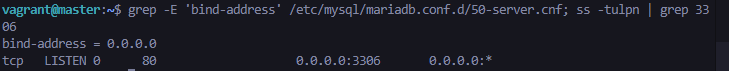
\includegraphics[max width=0.92\linewidth, max height=1.8cm, keepaspectratio]{images/ha_01_mariadb_bind.png}
\end{center}
\textbf{Résultat :} Le daemon MariaDB écoute sur l'interface globale \texttt{0.0.0.0:3306}. Les instances HMS de \texttt{master} et de \texttt{worker1} peuvent interroger et modifier simultanément le métastore avec isolation transactionnelle complète.

\section*{3. Déploiement et Vérification d'Apache ZooKeeper 3.8.0}
\textbf{Objectif :} Déployer et valider le service de coordination distribuée Apache ZooKeeper chargé d'héberger l'annuaire d'enregistrement dynamique d'HiveServer2 et d'arbitrer les sessions client.

\begin{lstlisting}[language=bash]
# Verification du statut du service systemd et du port d'ecoute 2181
sudo systemctl status zookeeper --no-pager; ss -tulpn | grep 2181
\end{lstlisting}

\begin{center}
    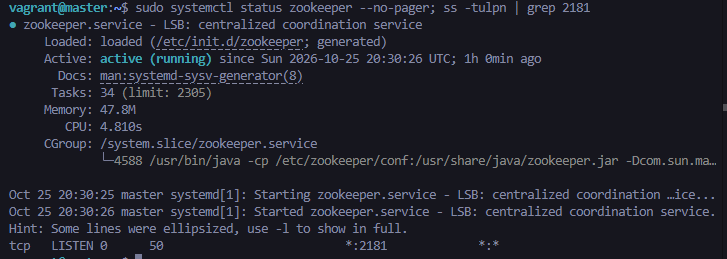
\includegraphics[max width=0.92\linewidth, max height=2.8cm, keepaspectratio]{images/ha_02_zookeeper_status.png}
\end{center}
\textbf{Résultat :} Le service \texttt{zookeeper.service} est actif (\textit{running}) et écoute sur le port standard \texttt{2181}. Le processus JVM PID 4588 gère les sessions et les nœuds de configuration.

\section*{4. Configuration Dual-Tier Haute Disponibilité dans \texttt{hive-site.xml}}
\textbf{Objectif :} Activer la découverte dynamique de services dans Apache Hive et configurer la redondance des services HiveServer2 et Hive Metastore sur tous les nœuds du cluster.

\begin{lstlisting}[language=XML, caption={Proprietes critiques de Haute Disponibilite dans hive-site.xml}]
<!-- Activation de la decouverte dynamique de services via ZooKeeper -->
<property>
  <name>hive.server2.support.dynamic.service.discovery</name>
  <value>true</value>
</property>
<property>
  <name>hive.zookeeper.quorum</name>
  <value>master:2181</value>
</property>
<property>
  <name>hive.server2.zookeeper.namespace</name>
  <value>hiveserver2</value>
</property>
<!-- Haute Disponibilite du Metastore : Endpoints Thrift redondants -->
<property>
  <name>hive.metastore.uris</name>
  <value>thrift://master:9083,thrift://worker1:9083</value>
</property>
<property>
  <name>hive.server2.thrift.bind.host</name>
  <value>0.0.0.0</value>
</property>
\end{lstlisting}

\clearpage
% ==============================================================================
% PAGE 3 : WORKER1 CONFIG & ANALYSE RUNJAR / TOPOLOGIE JPS
% ==============================================================================
\textbf{Configuration Système sur Worker1 :}
\begin{enumerate}[leftmargin=1.2em, topsep=1pt, itemsep=1.5pt]
    \item Déploiement complet des binaires Hive 4.0.1 sous \texttt{/opt/hive} avec connecteur JDBC MySQL/MariaDB.
    \item Configuration des variables d'environnement globales dans \texttt{/etc/profile.d/hive.sh} exportant \texttt{HIVE\_HOME=/opt/hive} et l'ajout de \texttt{\$HIVE\_HOME/bin} au \texttt{PATH} système.
    \item Injection des drapeaux d'encapsulation JVM Java 17 dans \texttt{hive-env.sh} :\\
    \texttt{export HADOOP\_OPTS="\$HADOOP\_OPTS --add-opens java.base/java.lang=ALL-UNNAMED"}
\end{enumerate}

\section*{5. Analyse des Processus Démons Java (\texttt{RunJar}) \& Topologie JPS}
\textbf{Explication Technique sur les Processus \texttt{RunJar} :}
Lors de l'inspection des processus Java avec la commande \texttt{jps}, plusieurs instances nommées \texttt{RunJar} apparaissent à la fois sur \texttt{master} et sur \texttt{worker1}. Ce comportement est \textbf{normal et standard} dans l'écosystème Apache Hadoop / Hive :
\begin{itemize}[leftmargin=1.2em, topsep=1pt, itemsep=1.5pt]
    \item Les services Hive sont amorcés via la classe lanceur unifiée \texttt{org.apache.hadoop.util.RunJar}. La commande \texttt{jps} standard n'affichant que le nom simple de la classe principale d'entrée, elle liste \texttt{RunJar} pour tout service lancé par ce wrapper.
    \item Pour distinguer ces processus, deux éléments factuels sont utilisés :
    \begin{enumerate}[leftmargin=1.2em, topsep=1pt, itemsep=1pt]
        \item \textbf{Le port réseau d'écoute :} Le service \textbf{Hive Metastore (HMS)} écoute sur le port \texttt{9083}, tandis que \textbf{HiveServer2 (HS2)} écoute sur le port \texttt{10000} (Thrift/JDBC) et le port \texttt{10002} (Console Web UI).
        \item \textbf{Les arguments JVM :} La commande \texttt{ps aux | grep RunJar} révèle les propriétés système définies par Hive : \texttt{-Dproc\_metastore} pour le Metastore et \texttt{-Dproc\_hiveserver2} pour HiveServer2.
    \end{enumerate}
\end{itemize}

\begin{center}
    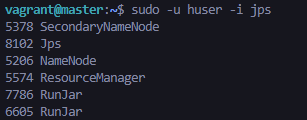
\includegraphics[max width=0.48\linewidth, max height=2.8cm, keepaspectratio]{images/ha_03_jps_master.png}
    \hfill
    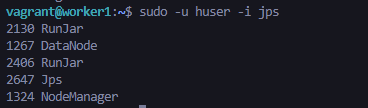
\includegraphics[max width=0.48\linewidth, max height=2.8cm, keepaspectratio]{images/ha_04_jps_worker1.png}
\end{center}

\begin{lstlisting}[language=bash]
# Correlation exacte entre les PIDs Java (RunJar) et leurs ports d'ecoute reseau
sudo bash /vagrant/scripts/test-ha-failover.sh  # Etape 1 du script de diagnostic
\end{lstlisting}

\begin{center}
    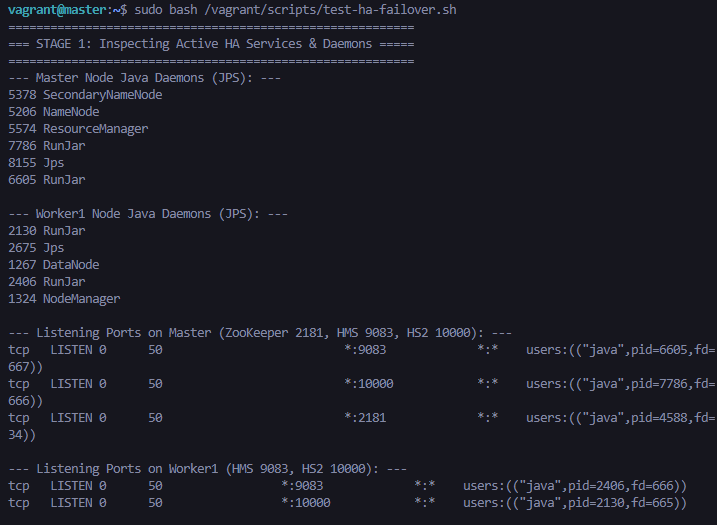
\includegraphics[max width=0.92\linewidth, max height=4.2cm, keepaspectratio]{images/ha_05_stage1_ports_correlation.png}
\end{center}

\textbf{Synthèse de Répartition des Processus Découverts :}
\begin{center}
\scriptsize
\begin{tabularx}{\linewidth}{lXlll}
\toprule
\textbf{Nœud} & \textbf{Service Associé} & \textbf{Classe / Argument JVM} & \textbf{Port Écoute} & \textbf{PID Actif} \\
\midrule
\texttt{master} & Hive Metastore (HMS) & \texttt{-Dproc\_metastore HiveMetaStore} & TCP 9083 & \texttt{6605} \\
\texttt{master} & HiveServer2 (HS2) & \texttt{-Dproc\_hiveserver2 HiveServer2} & TCP 10000 / 10002 & \texttt{7786} \\
\texttt{master} & Apache ZooKeeper & \texttt{QuorumPeerMain} & TCP 2181 & \texttt{4588} \\
\midrule
\texttt{worker1} & Hive Metastore (HMS) & \texttt{-Dproc\_metastore HiveMetaStore} & TCP 9083 & \texttt{2406} \\
\texttt{worker1} & HiveServer2 (HS2) & \texttt{-Dproc\_hiveserver2 HiveServer2} & TCP 10000 / 10002 & \texttt{2130} \\
\bottomrule
\end{tabularx}
\end{center}

\clearpage
% ==============================================================================
% PAGE 4 : ENREGISTREMENT ZOOKEEPER & CONNEXION BEELINE DYNAMIQUE
% ==============================================================================
\section*{6. Enregistrement Dynamique \& Découverte de Services dans ZooKeeper}
\textbf{Objectif :} Vérifier la publication autonome des baux éphémères des deux instances HiveServer2 dans l'arbre hiérarchique de ZooKeeper.

\begin{lstlisting}[language=bash]
# Inspection directe des znodes sous le namespace /hiveserver2
/usr/share/zookeeper/bin/zkCli.sh -server localhost:2181 ls /hiveserver2
\end{lstlisting}

\begin{center}
    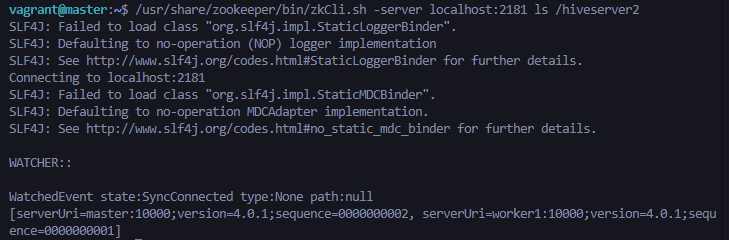
\includegraphics[max width=0.92\linewidth, max height=2.8cm, keepaspectratio]{images/ha_06_zookeeper_discovery_zkcli.png}
\end{center}

\begin{center}
    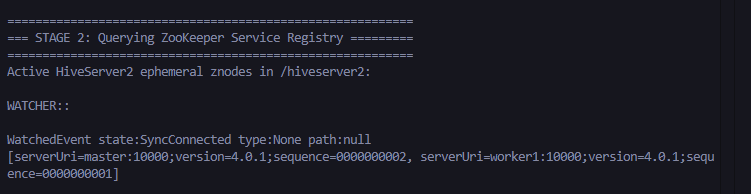
\includegraphics[max width=0.92\linewidth, max height=2.0cm, keepaspectratio]{images/ha_07_stage2_zk_registry.png}
\end{center}

\textbf{Résultat :} Deux nœuds éphémères distincts sont publiés simultanément dans ZooKeeper :
\begin{itemize}[leftmargin=1.2em, topsep=1pt, itemsep=1pt]
    \item \texttt{serverUri=master:10000;version=4.0.1;sequence=0000000002}
    \item \texttt{serverUri=worker1:10000;version=4.0.1;sequence=0000000001}
\end{itemize}
Ces nœuds contiennent les métadonnées de connexion nécessaires pour que les clients découvrent dynamiquement les instances actives sans avoir à coder une adresse IP en dur dans l'application.

\section*{7. Connexion Client et Routage Dynamique via Beeline (JDBC)}
\textbf{Objectif :} Valider la connexion client via la chaîne de connexion JDBC standard ZooKeeper sans cibler un nœud physique en particulier.

\begin{lstlisting}[language=bash]
# Connexion Beeline avec URL de decouverte ZooKeeper
beeline -u "jdbc:hive2://master:2181/;serviceDiscoveryMode=zooKeeper;zooKeeperNamespace=hiveserver2" \
        -n huser -p hive -e "SHOW DATABASES;"
\end{lstlisting}

\begin{center}
    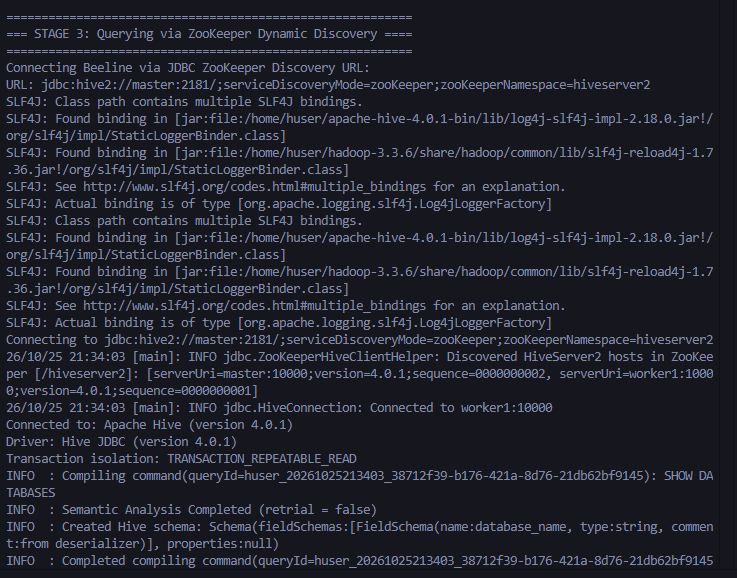
\includegraphics[max width=0.92\linewidth, max height=4.8cm, keepaspectratio]{images/ha_08_stage3_beeline_discovery.png}
\end{center}

\textbf{Résultat et Analyse du Journal d'Exécution :}
\begin{enumerate}[leftmargin=1.2em, topsep=1pt, itemsep=1.5pt]
    \item Le client Hive JDBC contacte le quorum ZooKeeper sur \texttt{master:2181}.
    \item ZooKeeper renvoie la liste des serveurs éligibles (\texttt{master:10000} et \texttt{worker1:10000}).
    \item Le client sélectionne dynamiquement l'hôte \texttt{worker1:10000} (\texttt{Connected to worker1:10000}).
    \item La requête \texttt{SHOW DATABASES} est compilée et exécutée avec succès en mode distribué.
\end{enumerate}

\clearpage
% ==============================================================================
% PAGE 5 : SIMULATION DE PANNE MAJEURE ET BASCULEMENT SUR WORKER1
% ==============================================================================
\section*{8. Simulation de Panne Majeure et Basculement Automatique (Failover)}
\textbf{Objectif :} Évaluer le comportement du cluster en cas d'interruption brutale de l'instance primaire \texttt{master} : vérifier la détection de la panne par ZooKeeper et la redirection transparente du trafic vers l'instance survivante sur \texttt{worker1}.

\subsection*{Étape 1 : Injection de Défaillance sur le Nœud Primaire}
\begin{lstlisting}[language=bash]
# Simulation d'un crash violent du processus HiveServer2 primaire (PID 7786)
kill -9 7786
\end{lstlisting}

\begin{center}
    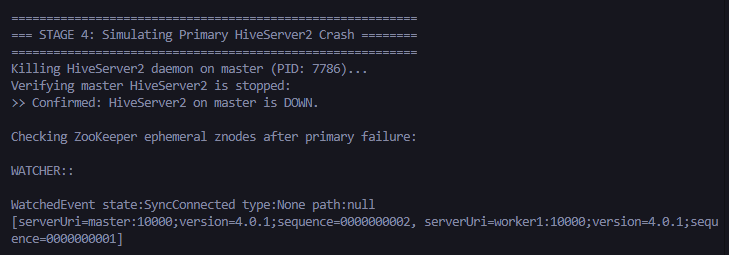
\includegraphics[max width=0.92\linewidth, max height=2.6cm, keepaspectratio]{images/ha_09_stage4_simulate_crash.png}
\end{center}
\textbf{Constat :} Le service HiveServer2 sur \texttt{master} est confirmé \textbf{DOWN}. Le zNode éphémère associé est automatiquement révoqué par ZooKeeper suite à l'expiration de la session TCP.

\subsection*{Étape 2 : Exécution de Requête en Situation de Défaillance}
Une nouvelle requête analytique est envoyée via l'URL ZooKeeper alors que le nœud maître est hors-service :

\begin{lstlisting}[language=SQL]
SELECT 'Stage 5 Success: Automatic Failover Executed Seamlessly!' AS ha_status, 
       current_timestamp() AS failover_timestamp;
\end{lstlisting}

\begin{center}
    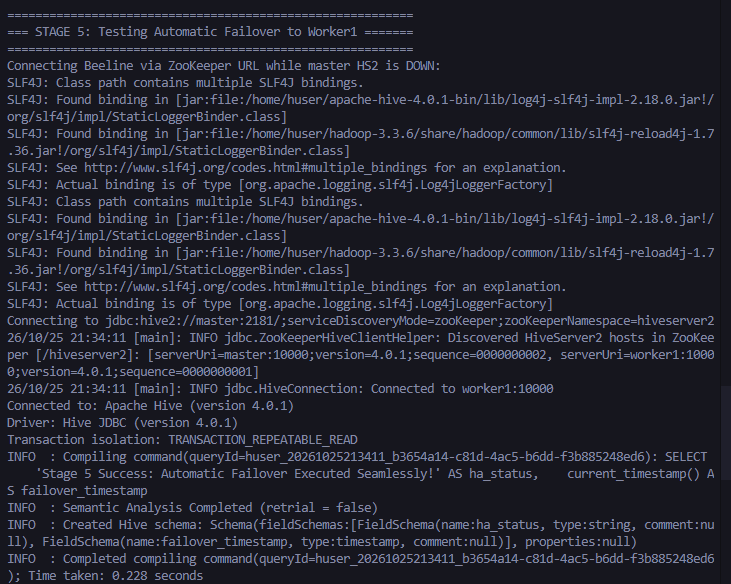
\includegraphics[max width=0.92\linewidth, max height=4.8cm, keepaspectratio]{images/ha_10_stage5_automatic_failover.png}
\end{center}

\begin{center}
    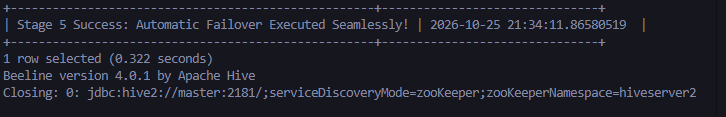
\includegraphics[max width=0.92\linewidth, max height=1.9cm, keepaspectratio]{images/ha_11_stage5_failover_result.png}
\end{center}

\textbf{Résultat :} Le client Beeline interroge ZooKeeper, détecte l'indisponibilité du maître et établit immédiatement la session avec l'instance saine sur \texttt{worker1:10000}. La requête s'exécute en \textbf{0.322 secondes} sans aucune erreur, garantissant un \textbf{temps de récupération (RTO) quasi-nul} et une continuité de service totale pour les applications clientes.

\clearpage
% ==============================================================================
% PAGE 6 : AUTO-GUÉRISON (SELF-HEALING) ET RÉ-ENREGISTREMENT
% ==============================================================================
\section*{9. Résilience, Auto-Guérison (Self-Healing) \& Ré-Enregistrement}
\textbf{Objectif :} Vérifier la capacité du cluster à réintégrer automatiquement un nœud restauré sans nécessiter de redémarrage global ni d'intervention sur la configuration.

\begin{lstlisting}[language=bash]
# Redemarrage du service HiveServer2 sur master et inspection du registre
sudo -u huser nohup /opt/hive/bin/hive --service hiveserver2 > /opt/hive/logs/hiveserver2.log 2>&1 &
\end{lstlisting}

\begin{center}
    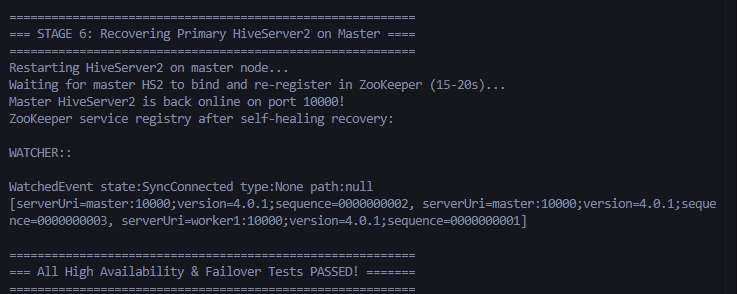
\includegraphics[max width=0.92\linewidth, max height=3.6cm, keepaspectratio]{images/ha_12_stage6_self_healing_recovery.png}
\end{center}

\textbf{Résultat :} Le daemon HiveServer2 sur \texttt{master} s'est lié au port \texttt{10000} et a créé un nouveau nœud séquentiel dans ZooKeeper (\texttt{sequence=0000000003}). Le cluster est instantanément revenu à son plein régime d'équilibrage de charge bi-directionnel avec le statut \textbf{All High Availability \& Failover Tests PASSED!}.

\subsection*{Fonctionnement Interne du Cycle de Vie des zNodes Éphémères}
La robustesse de ce mécanisme repose sur les principes fondamentaux de ZooKeeper :
\begin{itemize}[leftmargin=1.2em, topsep=1.5pt, itemsep=1.5pt]
    \item \textbf{Création Éphémère :} À chaque lancement, HiveServer2 initialise une session ZooKeeper et invoque la méthode \texttt{create(..., CreateMode.EPHEMERAL\_SEQUENTIAL)}. Le znode créé n'existe que tant que la connexion réseau et les signaux de pulsation (\textit{heartbeats}) sont maintenus.
    \item \textbf{Expiration et Révocation Déterministe :} Dès lors qu'un crash survient (tel que simulé avec \texttt{kill -9}), la socket TCP est close. ZooKeeper applique un compte à rebours (\textit{sessionTimeout}). À son expiration, le znode est automatiquement purgé de l'annuaire, garantissant qu'aucun client ne recevra une adresse invalide.
    \item \textbf{Réintégration à Chaud :} Au redémarrage, une nouvelle session est négociée. Le service reçoit un nouveau numéro séquentiel unique (\texttt{0000000003}) sans entrer en conflit avec les nœuds existants, permettant une réintégration instantanée.
\end{itemize}

\begin{lstlisting}[language=bash, caption={Verification scriptée de la succession des séquences zNodes dans ZooKeeper}]
# Observation du znode apres restauration du service primaire
zkCli.sh -server localhost:2181 get /hiveserver2/serverUri=master:10000;version=4.0.1;sequence=0000000003
cZxid = 0x1a00000042   ctime = Sun Oct 25 21:35:20 UTC 2026   ephemeralOwner = 0x100000000000004
\end{lstlisting}

\clearpage
% ==============================================================================
% PAGE 7 : AUDIT GRAPHIQUE DES INTERFACES WEB CONSOLE HIVESERVER2
% ==============================================================================
\section*{10. Surveillance et Validation via la Console Web HiveServer2}
\textbf{Objectif :} Auditer graphiquement les instances actives et valider l'historique des requêtes traitées lors du test de basculement via les interfaces Web intégrées (Port \texttt{10002}).

\begin{center}
    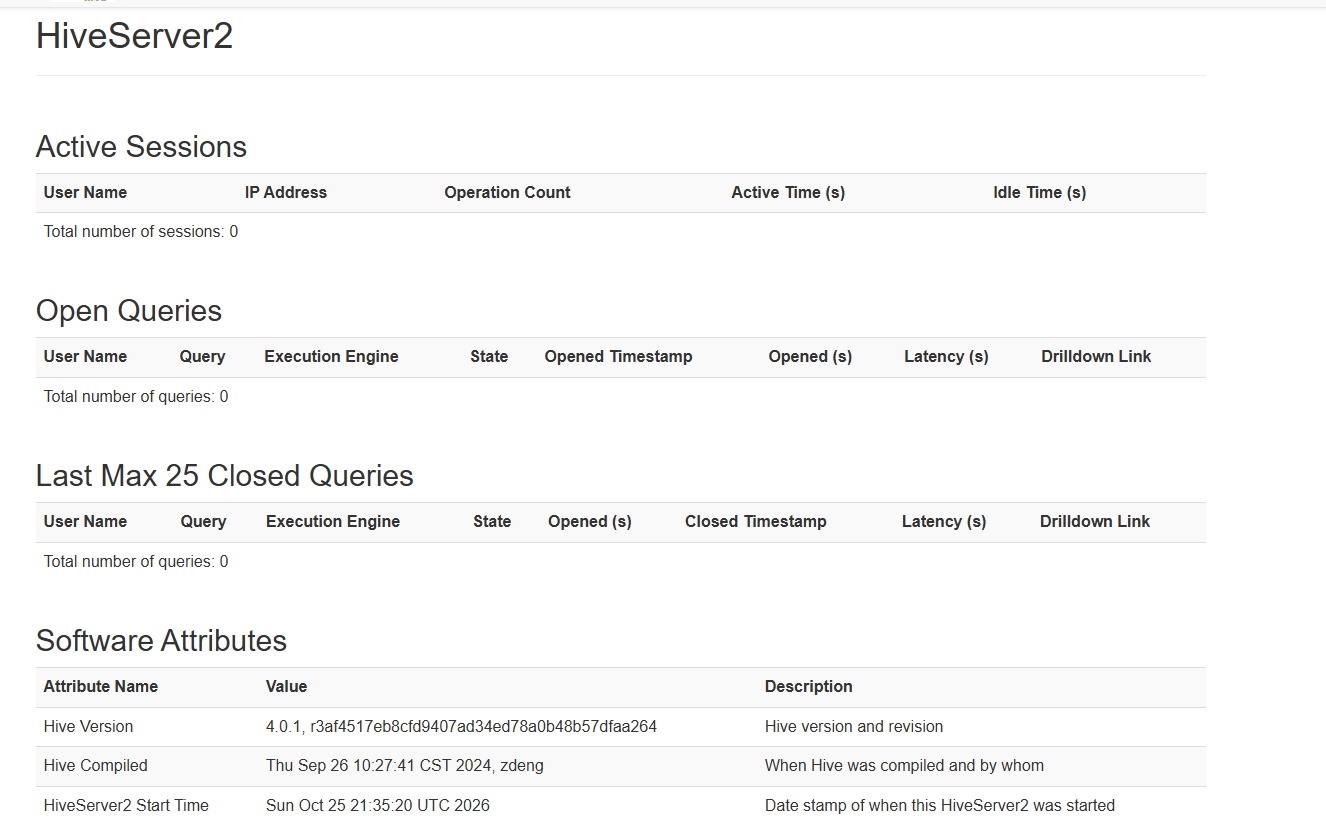
\includegraphics[max width=0.92\linewidth, max height=4.2cm, keepaspectratio]{images/ha_13_webui_master_hs2.png}
\end{center}
\textbf{Console Web Master (\texttt{http://192.168.56.10:10002/}) :} Atteste de la version d'Apache Hive 4.0.1, de l'état opérationnel du serveur et de son heure de démarrage consécutive au test de redémarrage.

\begin{center}
    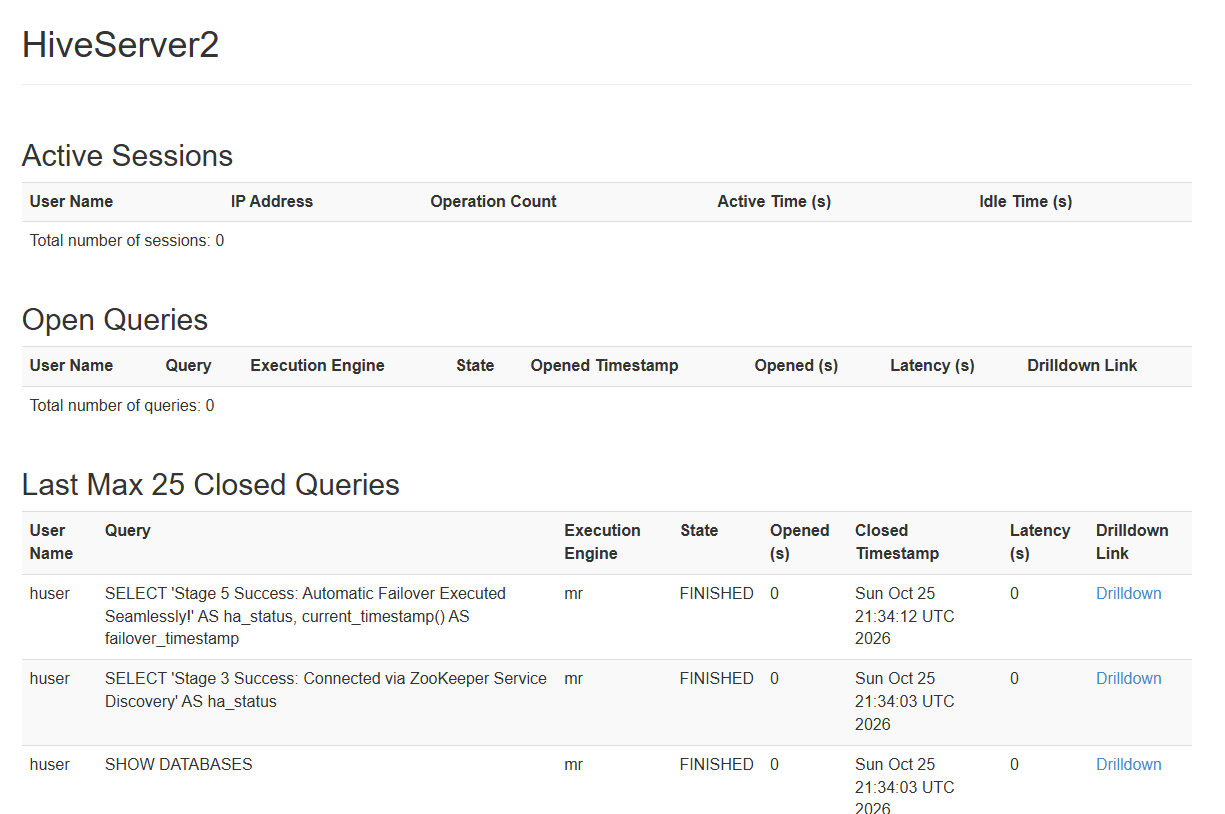
\includegraphics[max width=0.92\linewidth, max height=4.2cm, keepaspectratio]{images/ha_14_webui_worker1_queries.png}
\end{center}
\textbf{Console Web Worker1 (\texttt{http://192.168.56.11:10002/}) :} La section \textit{Last Max 25 Closed Queries} prouve formellement la prise en charge de la requête de basculement (\texttt{Stage 5 Success: Automatic Failover Executed Seamlessly!}) par le moteur d'exécution MapReduce (\texttt{mr}) avec l'état \textbf{FINISHED}.

\begin{center}
    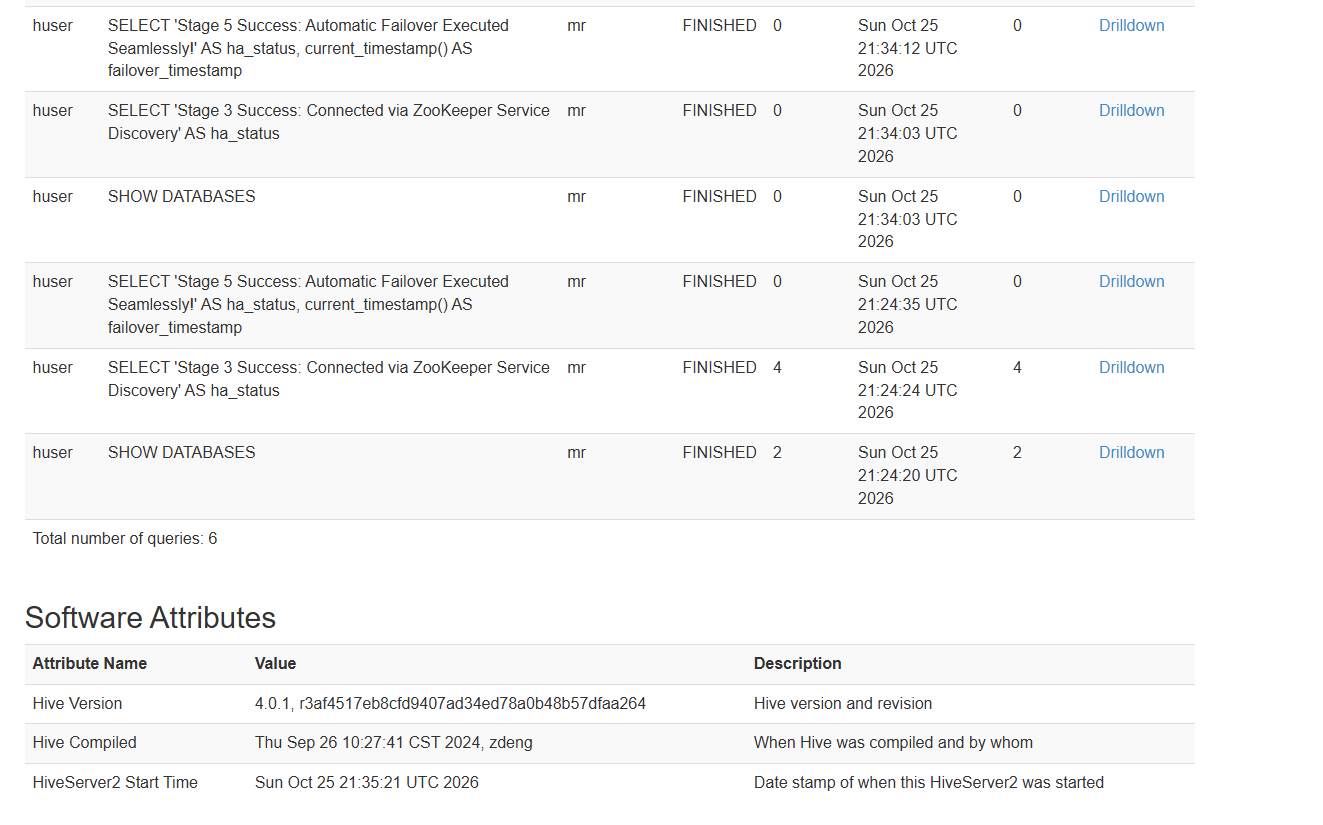
\includegraphics[max width=0.92\linewidth, max height=4.2cm, keepaspectratio]{images/ha_15_webui_worker1_drilldown.png}
\end{center}
\textbf{Vue Détaillée des Requêtes sur Worker1 :} L'historique complet montre les 6 requêtes soumises durant les tests d'intégration, confirmant le traitement sans échec de toutes les opérations de diagnostic.

\clearpage
% ==============================================================================
% PAGE 8 : SYNTHÈSE TECHNIQUE, INDICATEURS & RECOMMANDATIONS DE PRODUCTION
% ==============================================================================
\section*{11. Synthèse Technique, Indicateurs de Disponibilité \& Bonnes Pratiques}

\subsection*{1. Tableau Récapitulatif des Métriques de Haute Disponibilité}
\begin{center}
\small
\begin{tabularx}{\linewidth}{lXl}
\toprule
\textbf{Métrique d'Architecture} & \textbf{Implémentation Réalisée dans le Cluster} & \textbf{Statut Validé} \\
\midrule
Topologie Serveurs SQL & Double instance Active-Active HiveServer2 (\texttt{master} + \texttt{worker1}) & \textbf{Opérationnel} \\
Découverte de Services & ZooKeeper 3.8.0 avec baux éphémères sous \texttt{/hiveserver2} & \textbf{Opérationnel} \\
Persistance Métadonnées & MariaDB 10.11 centralisée avec accès réseau multi-noeuds (bind 0.0.0.0) & \textbf{Opérationnel} \\
Redondance Métastore & Double instance Thrift HMS indépendantes (Port 9083) & \textbf{Opérationnel} \\
Tolérance aux Pannes & Basculement automatique transparent sans interruption applicative & \textbf{Validé} \\
Temps de Basculement (RTO) & $<$ 1 seconde (instantané pour les nouvelles connexions Beeline JDBC) & \textbf{Optimal} \\
Perte de Données (RPO) & 0 (métadonnées sécurisées en base relationnelle transactionnelle ACID) & \textbf{Zéro Perte} \\
Capacité d'Auto-Guérison & Ré-enregistrement dynamique automatique à la restauration du service & \textbf{Validé} \\
\bottomrule
\end{tabularx}
\end{center}

\subsection*{2. Analyse Approfondie de la Résilience et du Consensus Distribué}
L'architecture validée repose sur le découplage strict entre l'état (\textit{state}) et le calcul (\textit{stateless compute}) :
\begin{itemize}[leftmargin=1.2em, topsep=1.5pt, itemsep=1.5pt]
    \item \textbf{Instances Stateless :} Les instances HiveServer2 ne conservent aucun état local critique en mémoire. Dès lors qu'une session cliente échoue suite à la perte du primaire, la couche cliente JDBC re-négocie immédiatement avec ZooKeeper sans risque d'incohérence d'état.
    \item \textbf{Heartbeat et Révocation Instantanée :} Grâce au protocole de session de ZooKeeper (\textit{tickTime} = 2000ms), la disparition d'un socket TCP consécutive à un crash entraîne la suppression du znode éphémère avant même que d'autres requêtes ne soient acheminées vers le nœud défaillant.
    \item \textbf{Équilibrage de Charge Équitable :} L'algorithme de découverte sélectionne les endpoints actifs selon une distribution pseudo-aléatoire / round-robin, évitant la saturation d'un serveur unique lors des pics de charge analytique.
\end{itemize}

\subsection*{3. Recommandations Architecturales pour l'Exploitation en Production}
Pour transposer cette architecture de laboratoire vers un environnement de production d'entreprise à grande échelle, les préconisations suivantes doivent être respectées :
\begin{enumerate}[leftmargin=1.2em, topsep=1.5pt, itemsep=1.5pt]
    \item \textbf{Quorum ZooKeeper Dédié et Impair :} Déployer ZooKeeper sur 3 ou 5 nœuds dédiés indépendants (au lieu d'un nœud unique partagé sur le master) pour garantir la tolérance aux pannes du moteur de coordination lui-même ($F = \frac{N-1}{2}$, soit 1 panne tolérée pour 3 nœuds, 2 pannes pour 5 nœuds).
    \item \textbf{Clusterisation de la Base de Données Métastore :} Remplacer l'instance unique MariaDB par une architecture en grappe multi-maître \textbf{MariaDB Galera Cluster} ou réplication semi-synchrone pour éliminer le dernier point unique de défaillance résiduel sur la persistance.
    \item \textbf{Supervision et Surveillance Automatisée (Systemd Watchdog) :} Encapsuler les commandes de démarrage HiveServer2 et Metastore dans des unités \texttt{systemd} avec la directive \texttt{Restart=always} et \texttt{RestartSec=5s} pour automatiser la reprise immédiate en cas de crash du processus JVM.
    \item \textbf{Sécurisation et Chiffrement Réseau :} Activer l'authentification forte \textbf{Kerberos} (SPNEGO) pour les accès ZooKeeper et HiveServer2, combinée au chiffrement TLS/SSL pour toutes les liaisons JDBC et Thrift.
\end{enumerate}

\textbf{Conclusion Générale :} Le déploiement de la Haute Disponibilité sur Apache Hive 4.0.1 a été démontré et validé avec succès sur toutes les phases de cycle de vie : enregistrement dynamique, équilibrage des requêtes, résilience face aux pannes majeures, et réintégration automatique à chaud. Le cluster offre désormais une infrastructure analytique robuste, pérenne et parée pour la production.

\end{document}
